\section{類似画像検索の実験結果}
自身の学籍番号の下二桁(01)と同じ下二桁の図形番号(ファイル名)を持つ画像を検索キー
(入力画像)としたときの検索結果(8個すべての特徴量を用いて検索し上位10位まで)を
示す。

\begin{itemize}
  \item[→] 以下の図\ref{graph:35}から図\ref{graph:45}は、私の学籍番号の下二桁(01)と同じ下二桁の図形番号を持つ画像をキーとした時の検索結果である。
  また、以下の表\ref{table:2}は、私の学籍番号の下二桁(01)と同じ下二桁の図形番号を持つ画像をキーとした時の検索結果の表である。
\end{itemize}

\begin{figure}[htbp]
  \begin{flushright}
    \begin{minipage}[t]{0.16\hsize}
      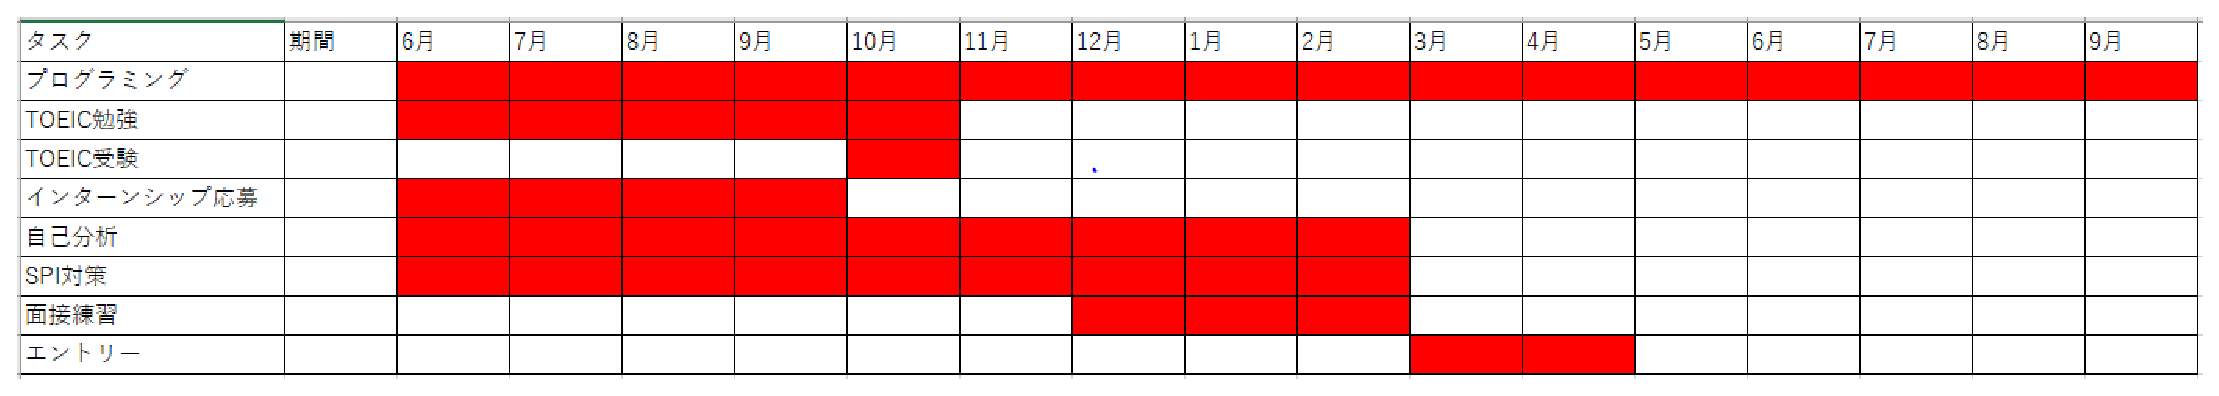
\includegraphics[scale=0.3]{img/1.bmp}
      \centering
      \caption{検索キー}
      \label{graph:35}
    \end{minipage}
    \begin{minipage}[t]{0.16\hsize}
      \includegraphics[scale=0.3]{img/3.bmp}
      \centering
      \caption{第1位}
      \label{graph:36}
    \end{minipage}
    \begin{minipage}[t]{0.16\hsize}
      \includegraphics[scale=0.3]{img/75.bmp}
      \centering
      \caption{第2位}
      \label{graph:37}
    \end{minipage}
    \begin{minipage}[t]{0.16\hsize}
      \includegraphics[scale=0.3]{img/74.bmp}
      \centering
      \caption{第3位}
      \label{graph:38}
    \end{minipage}
    \begin{minipage}[t]{0.16\hsize}
      \includegraphics[scale=0.3]{img/2.bmp}
      \centering
      \caption{第4位}
      \label{graph:39}
    \end{minipage}
    \begin{minipage}[t]{0.16\hsize}
      \includegraphics[scale=0.3]{img/12.bmp}
      \centering
      \caption{第5位}
      \label{graph:40}
    \end{minipage}
    \begin{minipage}[t]{0.16\hsize}
      \includegraphics[scale=0.3]{img/71.bmp}
      \centering
      \caption{第6位}
      \label{graph:41}
    \end{minipage}
    \begin{minipage}[t]{0.16\hsize}
      \includegraphics[scale=0.3]{img/9.bmp}
      \centering
      \caption{第7位}
      \label{graph:42}
    \end{minipage}
    \begin{minipage}[t]{0.16\hsize}
      \includegraphics[scale=0.3]{img/4.bmp}
      \centering
      \caption{第8位}
      \label{graph:43}
    \end{minipage}
    \begin{minipage}[t]{0.16\hsize}
      \includegraphics[scale=0.3]{img/10.bmp}
      \centering
      \caption{第9位}
      \label{graph:44}
    \end{minipage}
    \begin{minipage}[t]{0.16\hsize}
      \includegraphics[scale=0.3]{img/6.bmp}
      \centering
      \caption{第10位}
      \label{graph:45}
    \end{minipage}
  \end{flushright}
\end{figure}

\begin{table}[hbtp]
  \begin{tabular}{ccc}
    \begin{minipage}[t]{\hsize}
    \centering
    \caption{画像特徴量の計算結果}
    \label{table:2}
      \begin{tabular}{|c|c|c|}
        \hline
        順位 & 図形番号 & 検索キーとの距離\\
        \hline
        検索キー & 1 & 0 \\
        1 & 3 & 0.415 \\
        2 & 75 & 0.854 \\
        3 & 74 & 0.935 \\
        4 & 2 & 1.088 \\
        5 & 12 & 1.162 \\
        6 & 71 & 1.287 \\
        7 & 9 & 1.377 \\
        8 & 4 & 1.432 \\
        9 & 10 & 1.581 \\
        10 & 6 & 1.694 \\
        \hline
      \end{tabular}
    \end{minipage}
    
  \end{tabular}
\end{table}